
\documentclass[a4paper,12pt]{article}
\usepackage{graphicx}
\usepackage[table,xcdraw]{xcolor}
\usepackage{geometry}
\usepackage{float}
\usepackage[colorlinks=false, hidelinks]{hyperref}
\usepackage{fancyhdr}% For page numbering
\geometry{top=1in,bottom=1in,left=1in,right=1in}
\usepackage{listings}
\usepackage{xcolor}
\usepackage{hyperref}
\pagestyle{empty}


\begin{document}

\begin{center}
    \vspace{0.2cm}
    \textbf{\large{Course Title: Software Engineering \& ISD Lab}}\\
    \vspace{0.2cm}
    \textbf{Course Code: CSE-404}\\
    \vspace{0.2cm}
    \textbf{4\textsuperscript{th}Year 1\textsuperscript{st}Semester Examination 2023}\\
    \vspace{0.5cm}
    \textbf{Date of Submission: \today}\\

    \vspace{1.5cm}
    
\includegraphics[width=0.35\textwidth]{images/logo.png}\\ % Replace 'logo.png' with the correct path if you have the university logo image
    \vspace{1cm}

    \textbf{Submitted to}\\
    \vspace{0.2cm}
    \textbf{\href{https://juniv.edu/teachers/musfique.anwar}{Dr. Md Musfique Anwar}}\\
    {Professor}\\
    \vspace{0.2cm}
    \textbf{\href{https://juniv.edu/teachers/hkabir}{Dr. Md. Humayun Kabir}}\\
    {Professor}\\


    \vspace{1cm}

    \begin{table}[h!]
        \centering
        \arrayrulecolor{black}
        \begin{tabular}{|c|c|c|c|}
            \hline
            \rowcolor[HTML]{2F4F4F} % Changed header background color to dark slate gray
            {\color[HTML]{FFFFFF}\textbf{Sl}}& {\color[HTML]{FFFFFF}\textbf{Class Roll}}& {\color[HTML]{FFFFFF}\textbf{Exam Roll}}& {\color[HTML]{FFFFFF}\textbf{Name}}\\ \hline
            \rowcolor[HTML]{B0E0E6}
            \textbf{1}& \textbf{408} & \textbf{202220} & \textbf{Sudipta Singha} \\ \hline
       
        \end{tabular}
    \end{table}

    \vspace{1cm}

    Department of Computer Science and Engineering\\
    Jahangirnagar University\\
    Savar, Dhaka, Bangladesh\\
\end{center}

\newpage

\tableofcontents

\newpage
\pagestyle{fancy}
\fancyhf{}
\fancyfoot[C]{\thepage} % Page number in the center of the footer
\section{Sprint Overview}
This sprint's objective was to create the Jahangirnagar University Medical Center Management System's basic
features, with an emphasis on patient management, user access, and critical services. The team's goal was to
have basic functionality available by the conclusion of the sprint, such as the ability to create an account
and log in, schedule patient appointments, publish information about seasonal diseases, dispensing
medications, rescheduling tests, and viewing ambulance information. These characteristics will facilitate
early system interactions and offer a useful foundation for future advancements. During this sprint, I participated as a team member, contributing to coding, documentation, and discussions.
\newpage
\section{Sprint Review}
\subsection{Feature Demonstrated}
\begin{itemize}
    \item \textbf{Initial Authentication System: }Basic sign-up and login functionality with secure user session management.
    \item \textbf{Dashboard Framework: }Skeleton structure for the admin dashboard.
    \item \textbf{User Story Implementation: }
        \begin{itemize}
            \item Account creation for new users.
            \item Dispensing medicines to patients.
            \item Updating stock information.
        \end{itemize}
\end{itemize}
\subsection{Screenshots}
\begin{figure}[H]
    \centering
    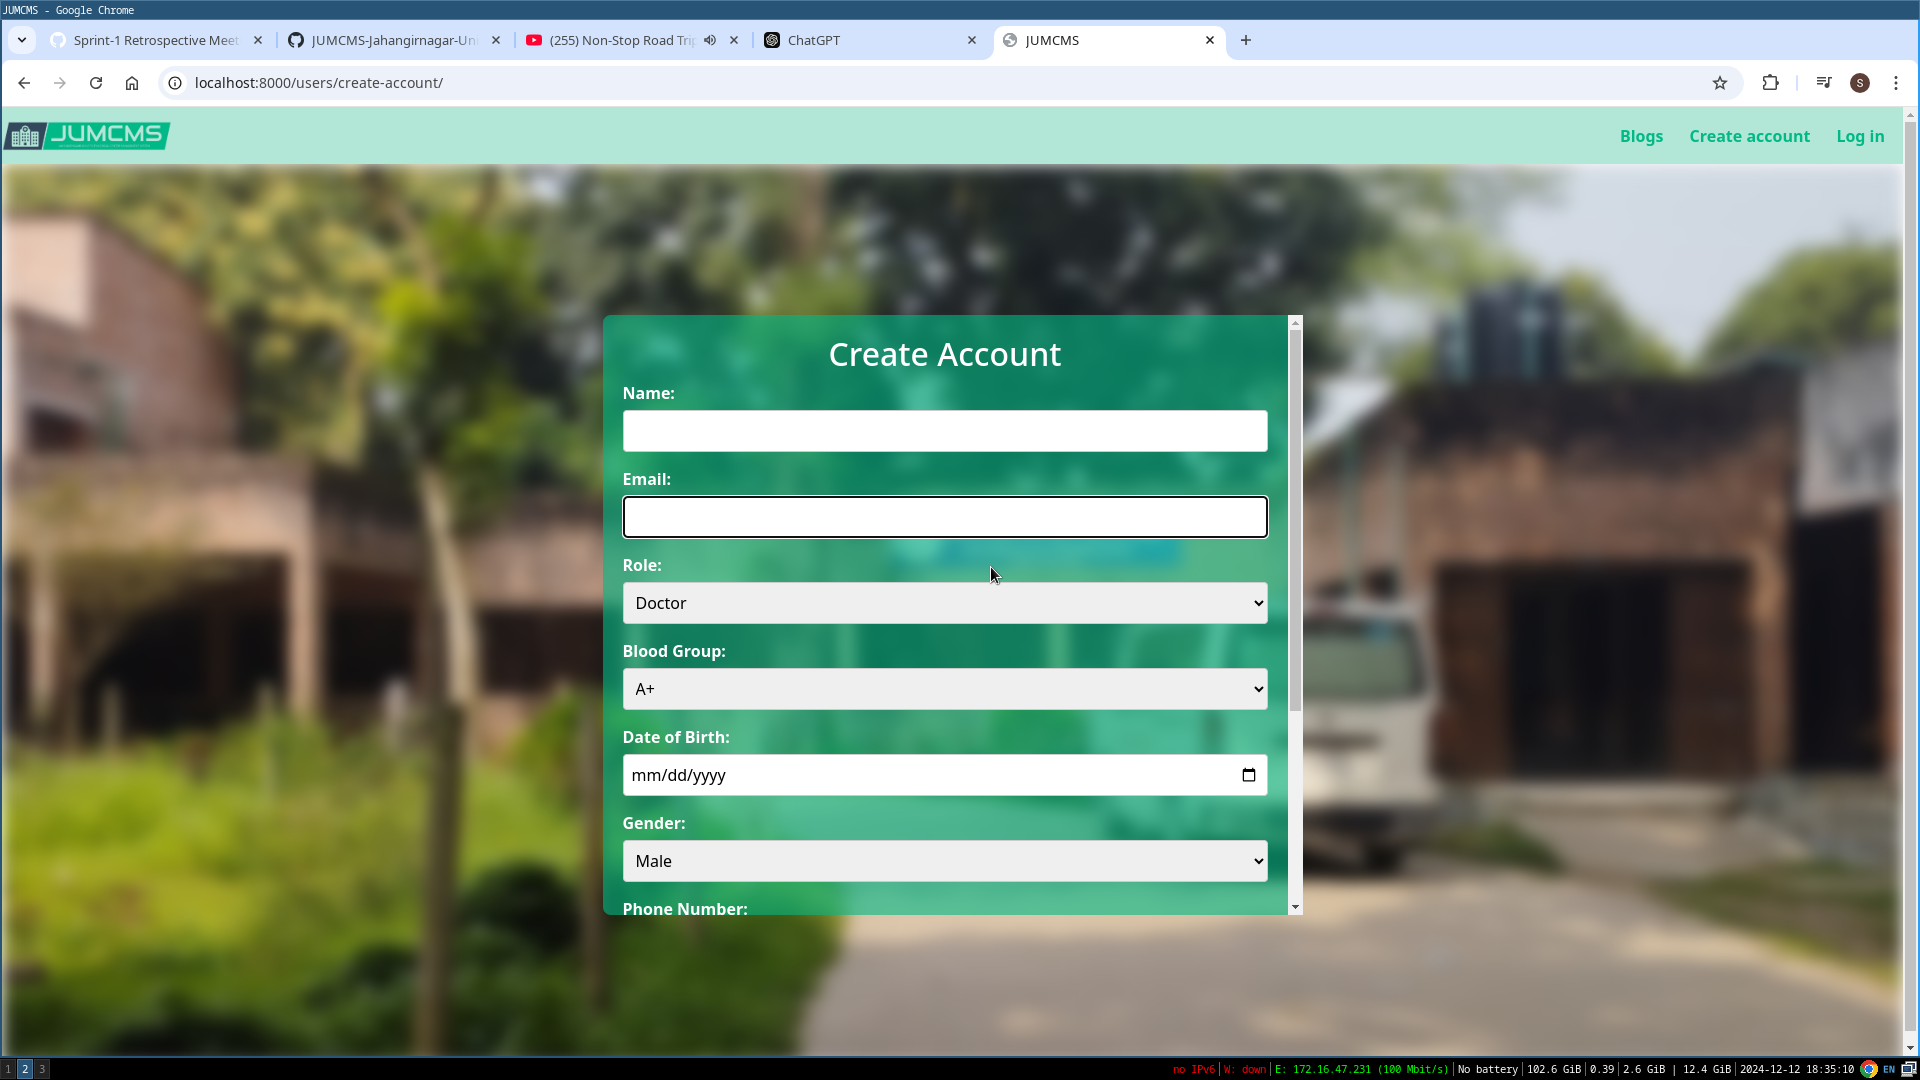
\includegraphics[width=1\textwidth]{images/spr1output2.png}
    \caption{Account Creation form}
    \label{fig:accountcreation}
\end{figure}

\begin{figure}[H]
    \centering
    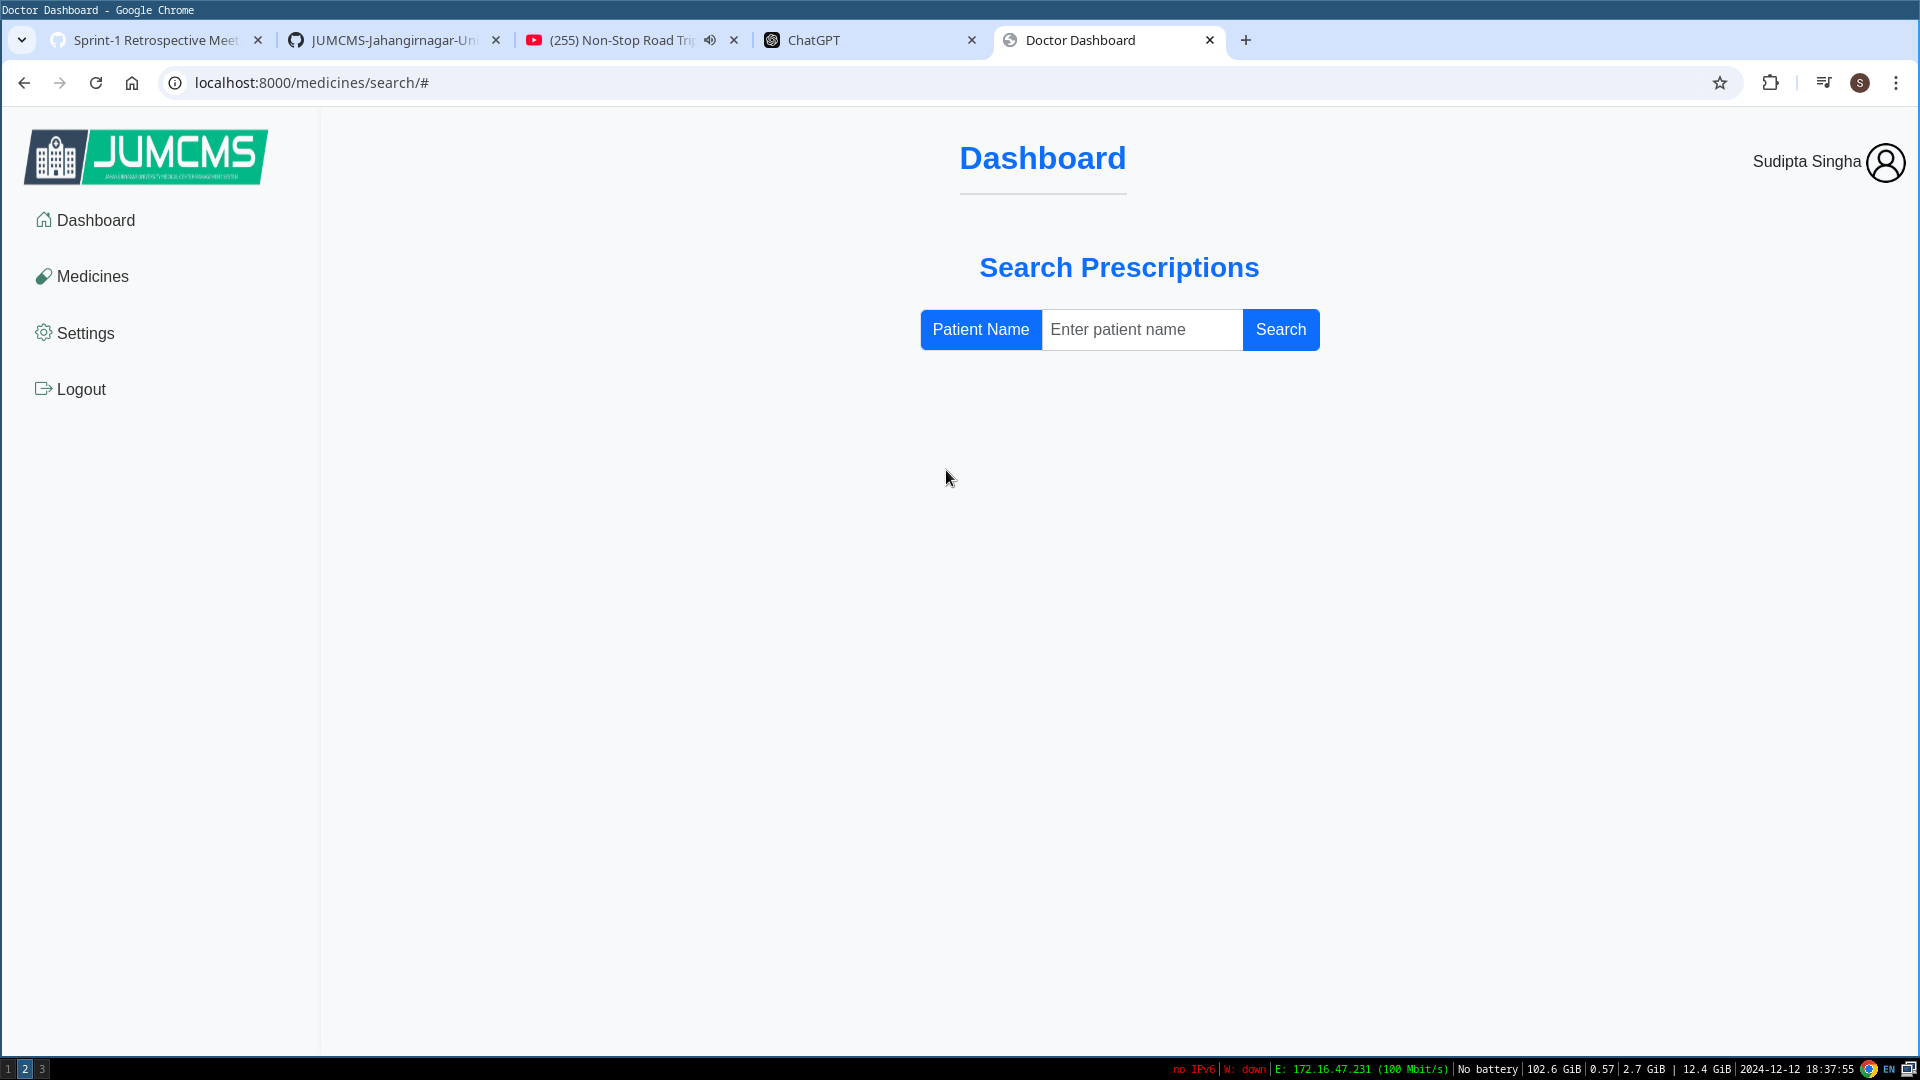
\includegraphics[width=1\textwidth]{images/spr1output3.png}
    \caption{Storekeeper Dashboard}
    \label{fig:storekeeperdashboard}
\end{figure}

\begin{figure}[H]
    \centering
    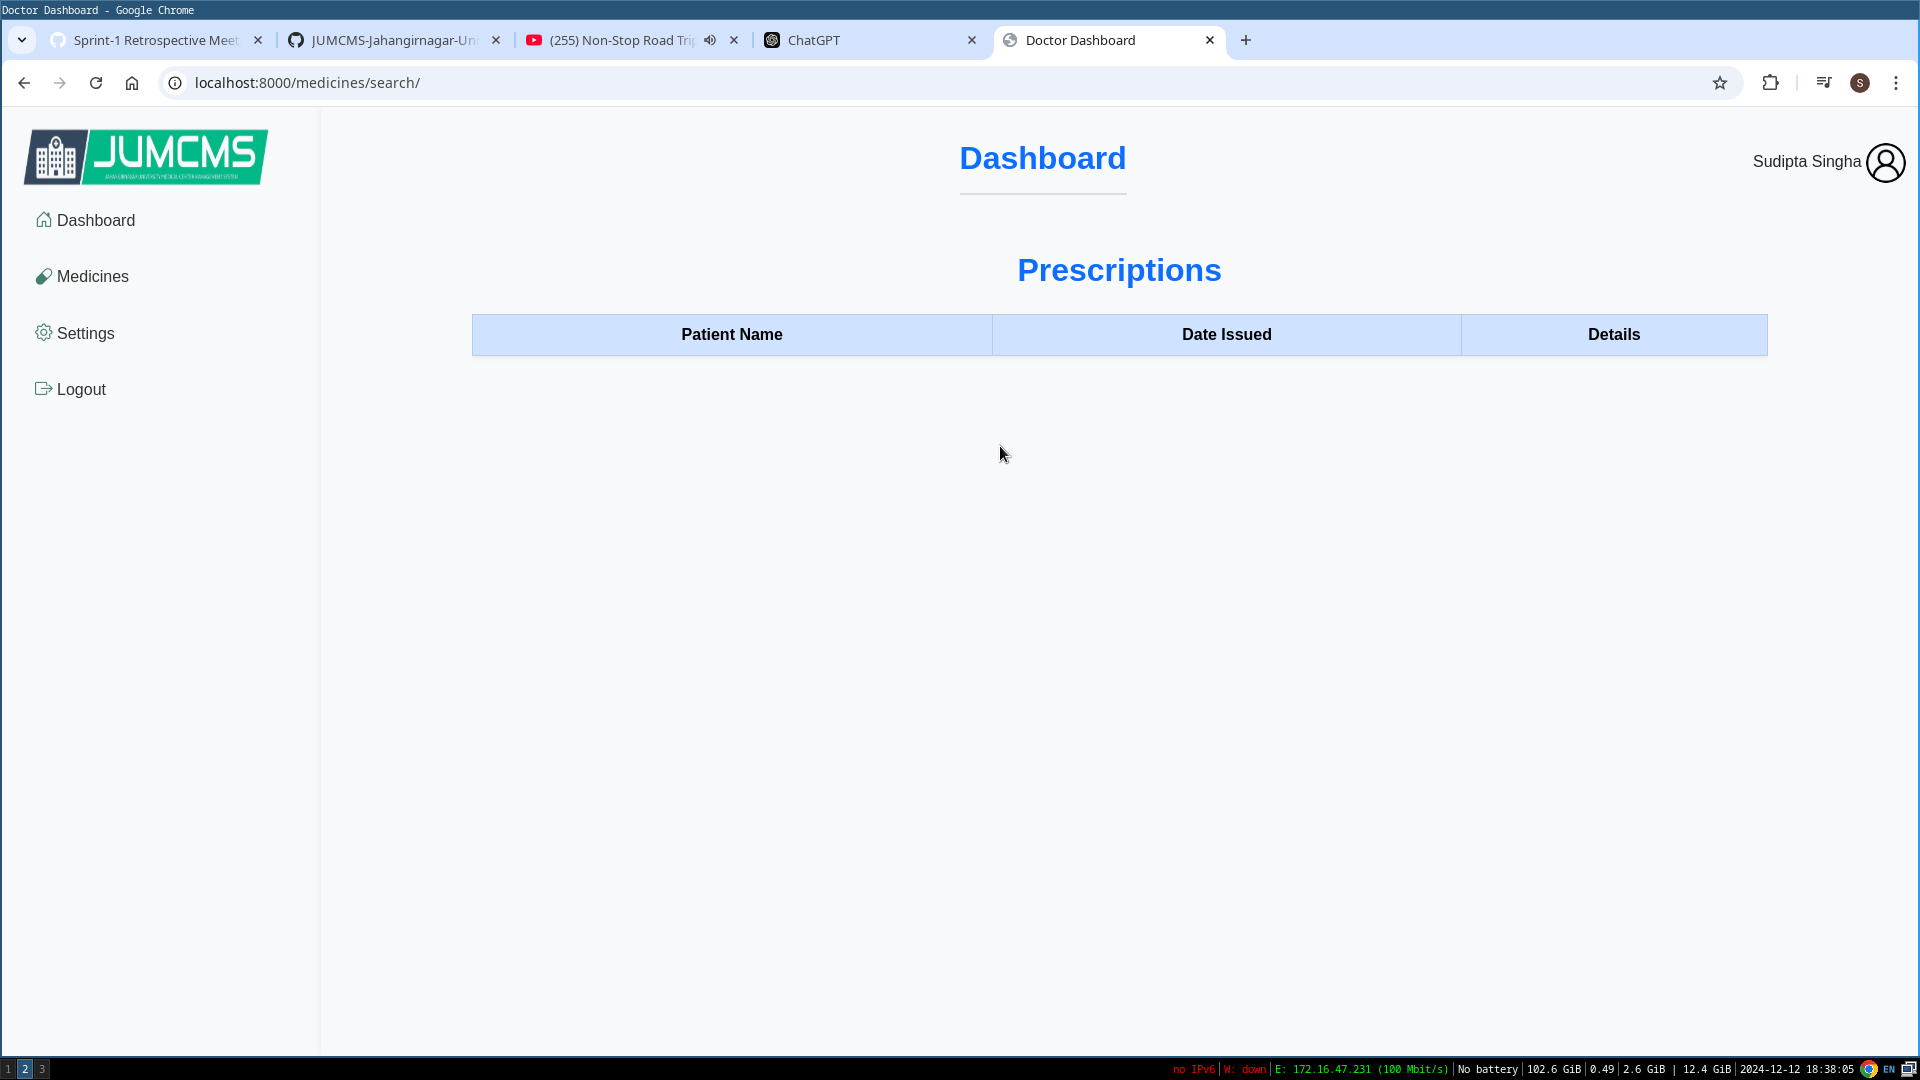
\includegraphics[width=1\textwidth]{images/spr1output4.png}
    \caption{Prescription List}
    \label{fig:prescriptionlist}
\end{figure}
\begin{figure}[H]
    \centering
    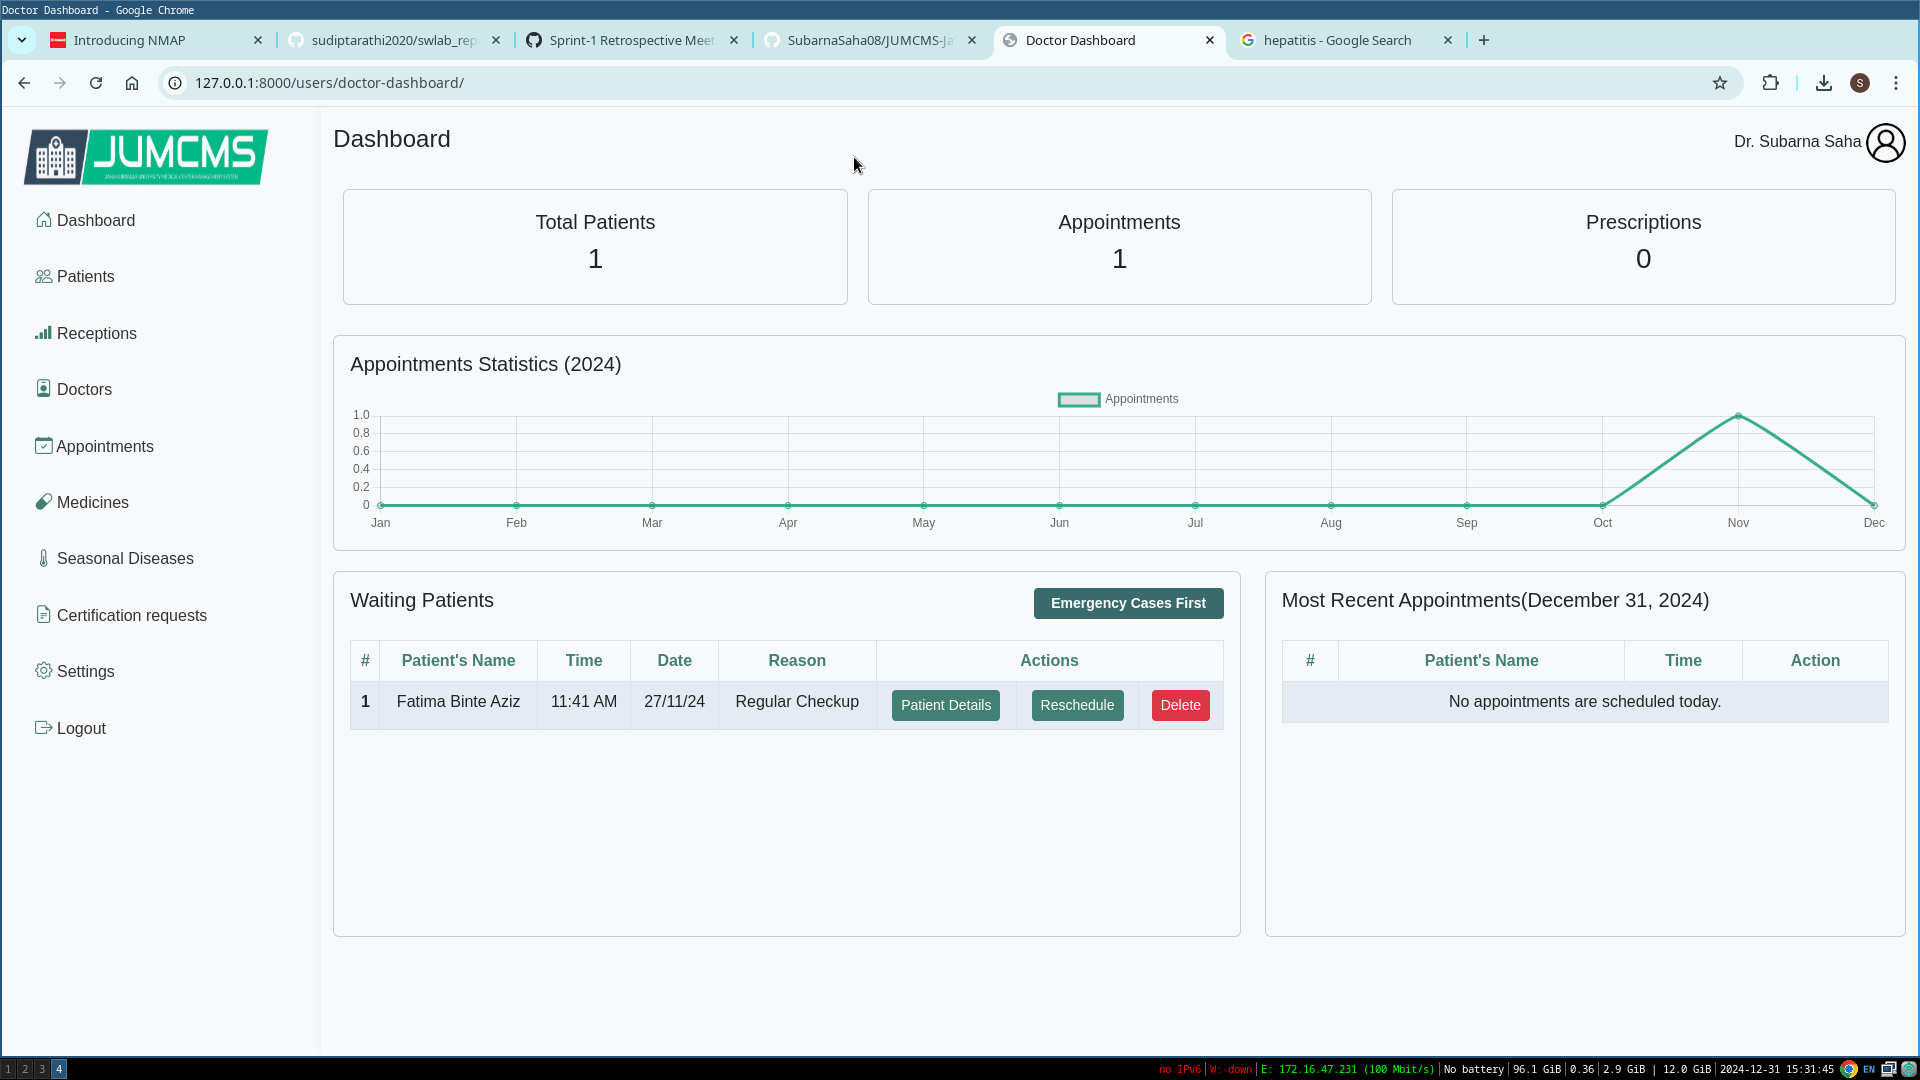
\includegraphics[width=1\textwidth]{images/sprintoutput01.png}
    \caption{Doctor Dashboard}
    \label{fig:doctordashboard}
\end{figure}

\begin{figure}[H]
    \centering
    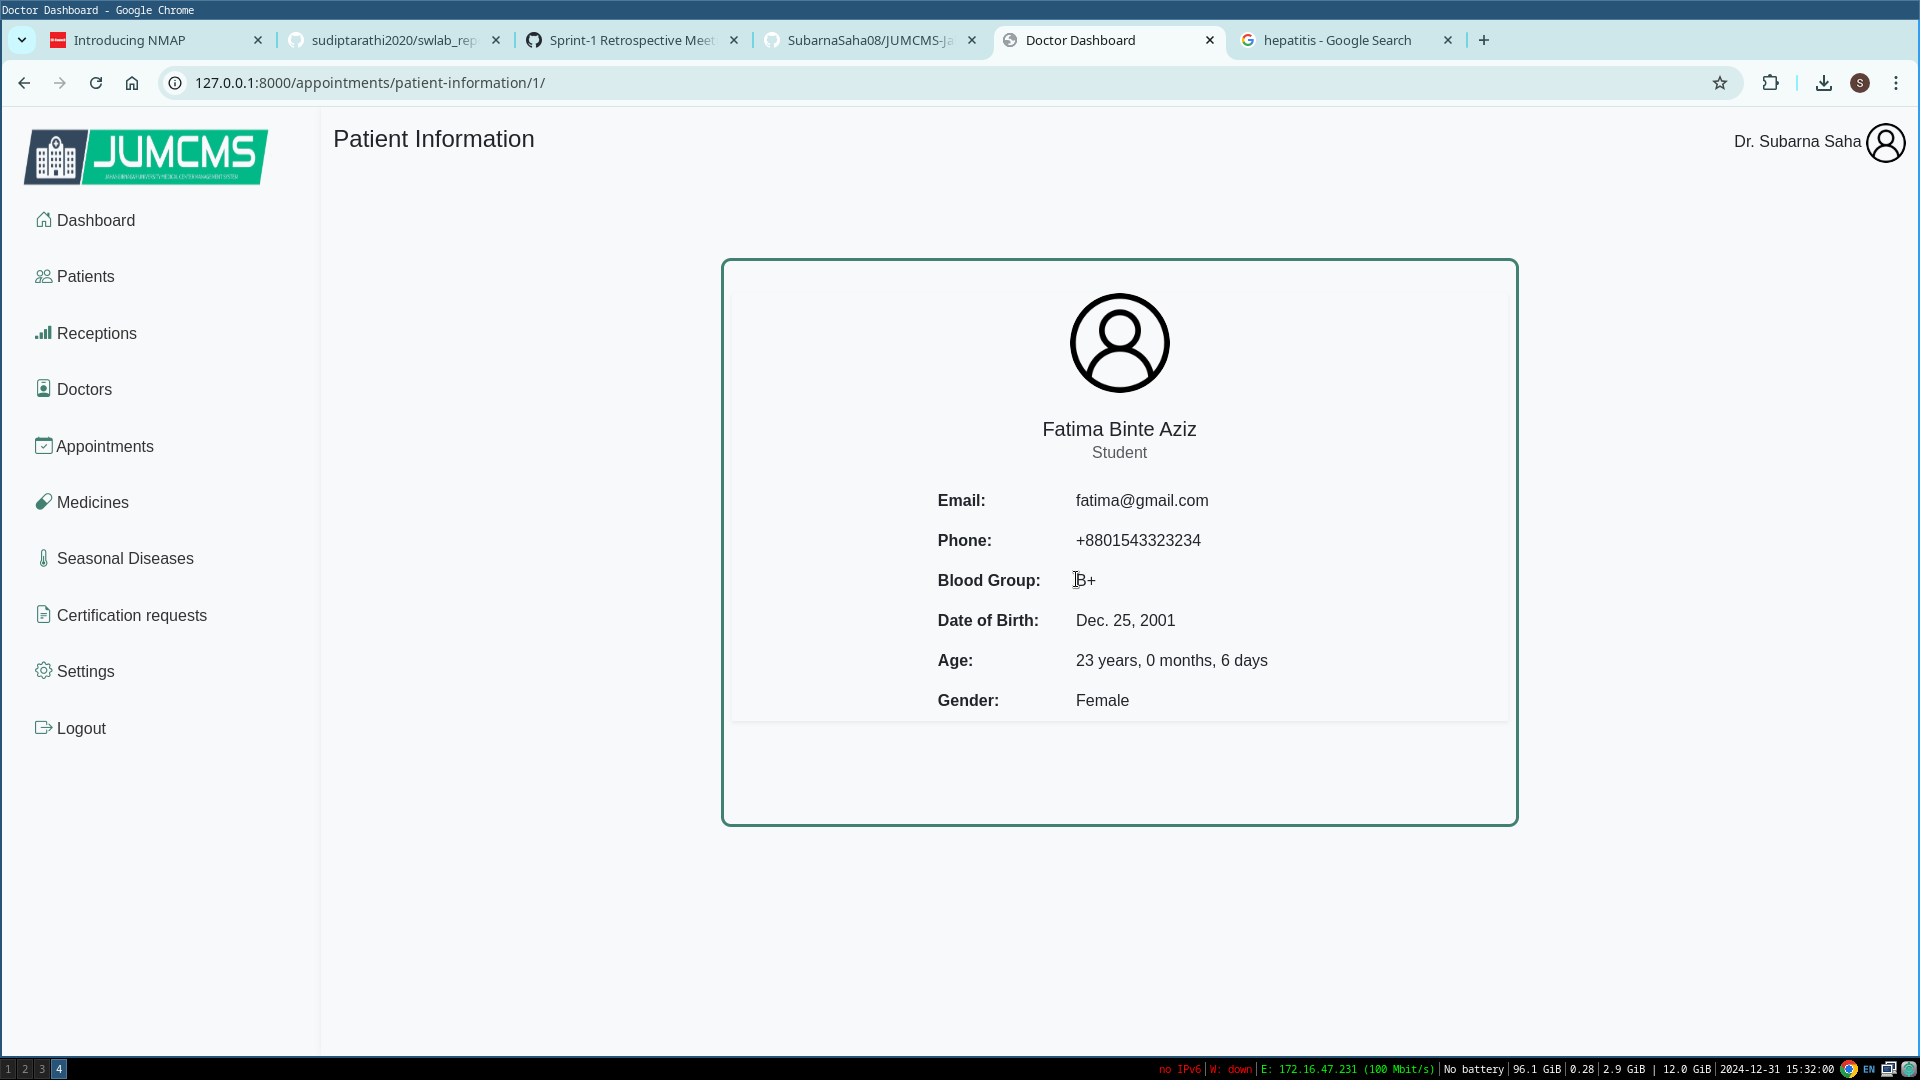
\includegraphics[width=1\textwidth]{images/sprintoutput02.png}
    \caption{Patient Details}
    \label{fig:patientdetails}
\end{figure}

\begin{figure}[H]
    \centering
    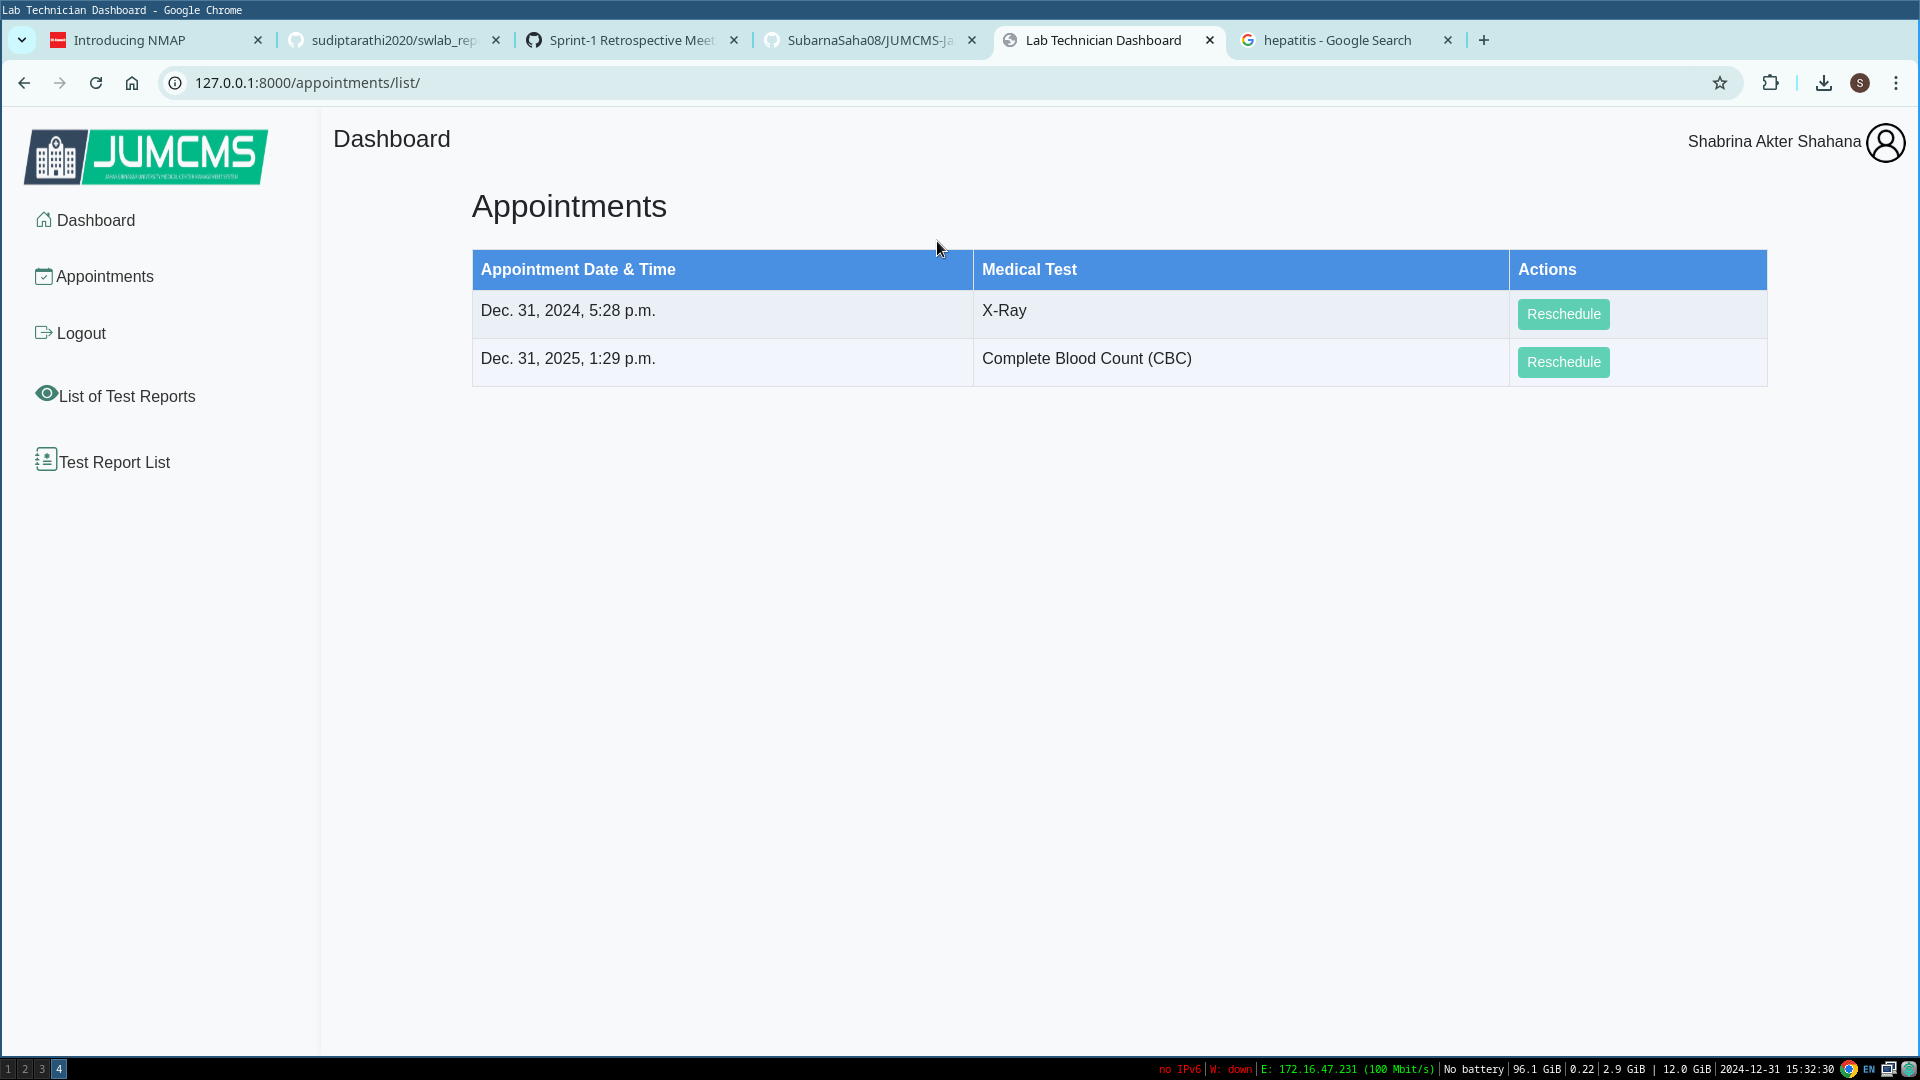
\includegraphics[width=1\textwidth]{images/sprintoutput03.png}
    \caption{Lab Technician Dashboard}
    \label{fig:labtechniciandashboard}
\end{figure}

\begin{figure}[H]
    \centering
    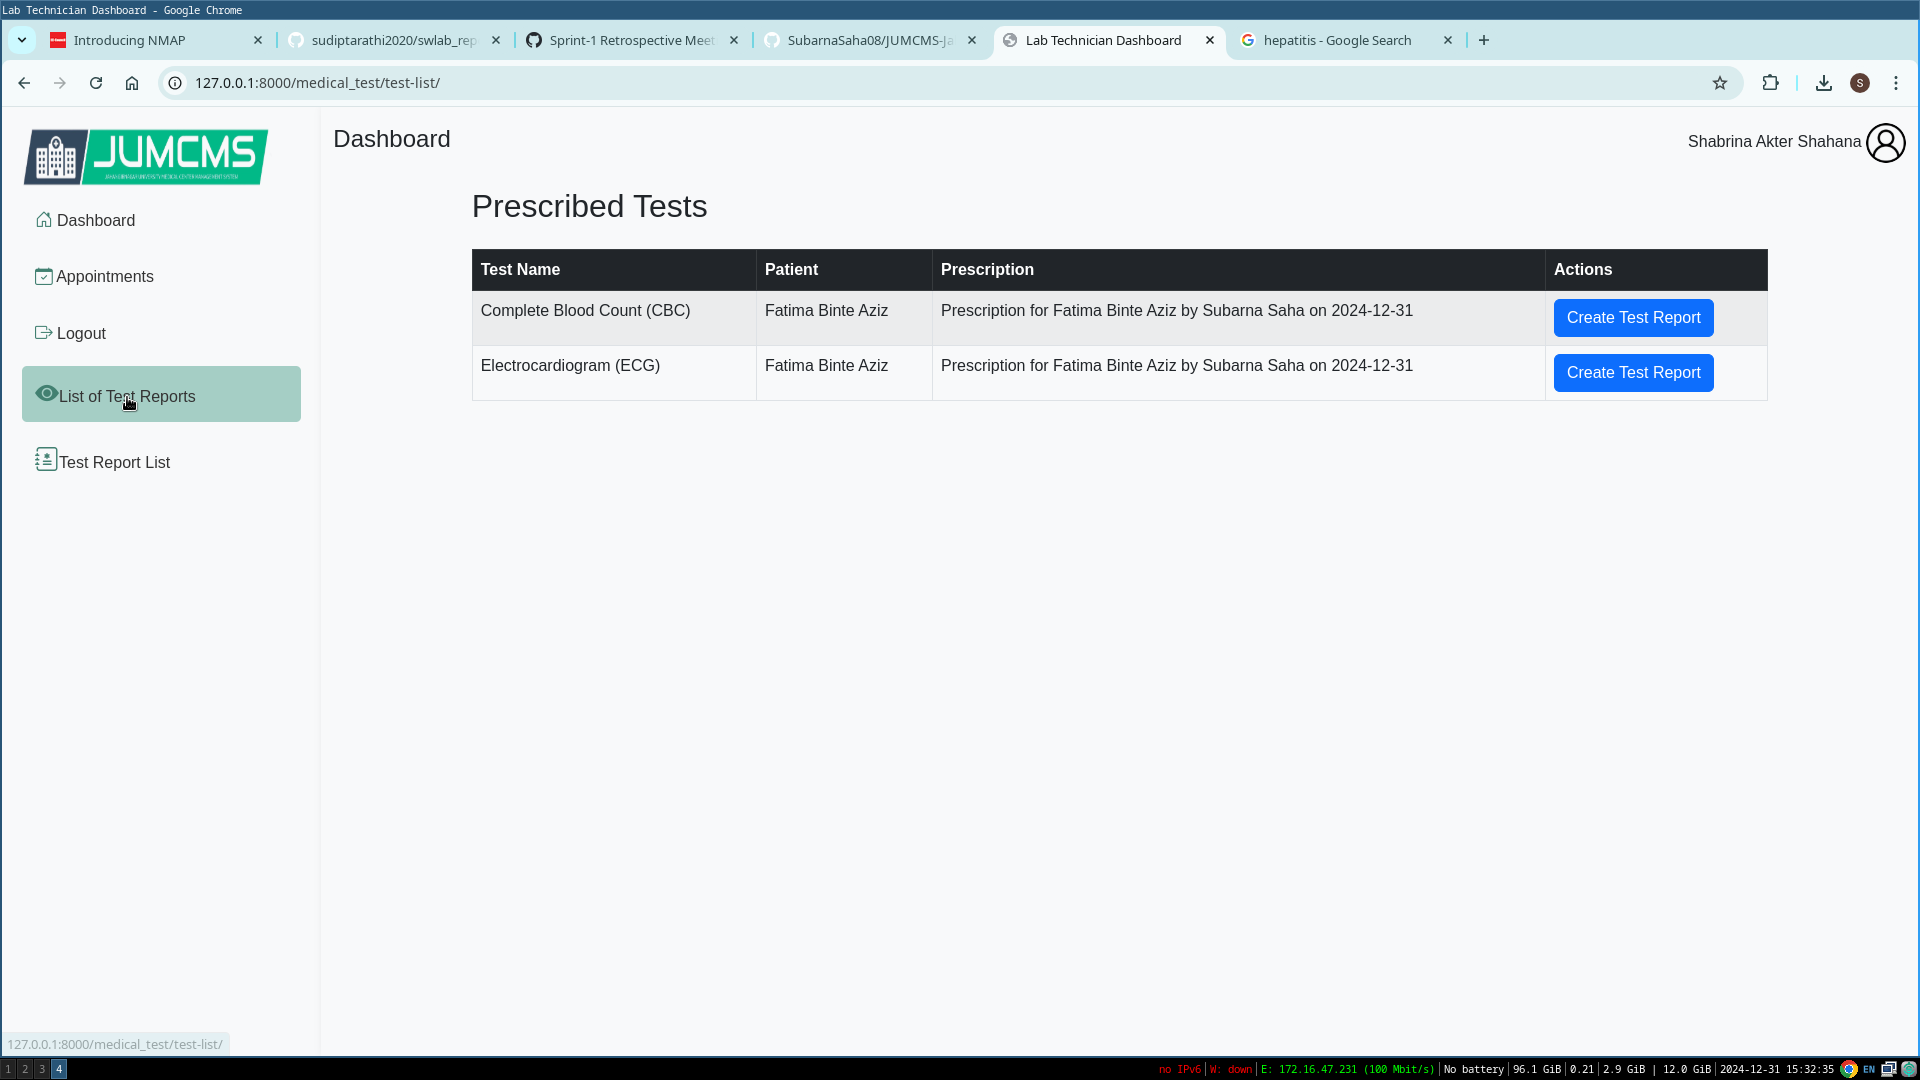
\includegraphics[width=1\textwidth]{images/sprintoutput05.png}
    \caption{Test Report Creation}
    \label{fig:reportcreation}
\end{figure}

\begin{figure}[H]
    \centering
    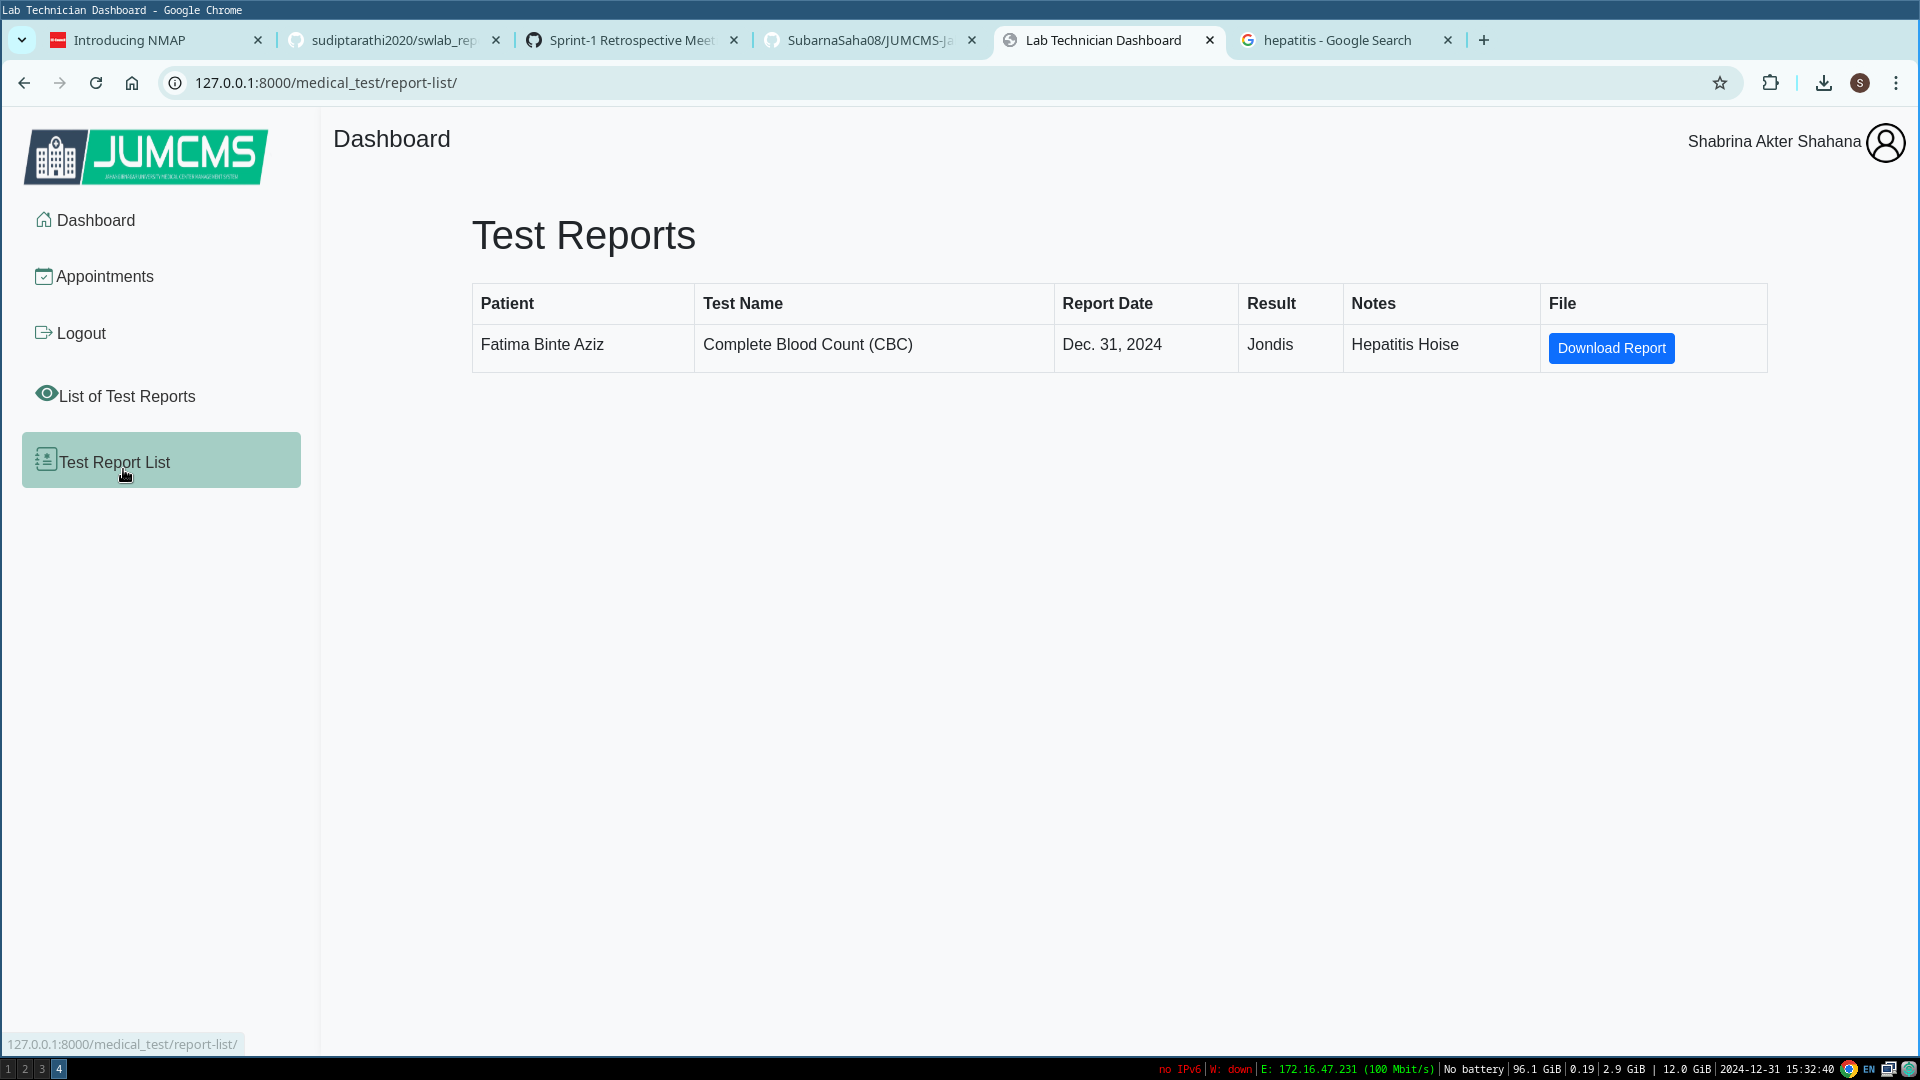
\includegraphics[width=1\textwidth]{images/sprintoutput06.png}
    \caption{List of Reports}
    \label{fig:reportlist}
\end{figure}

\begin{figure}[H]
    \centering
    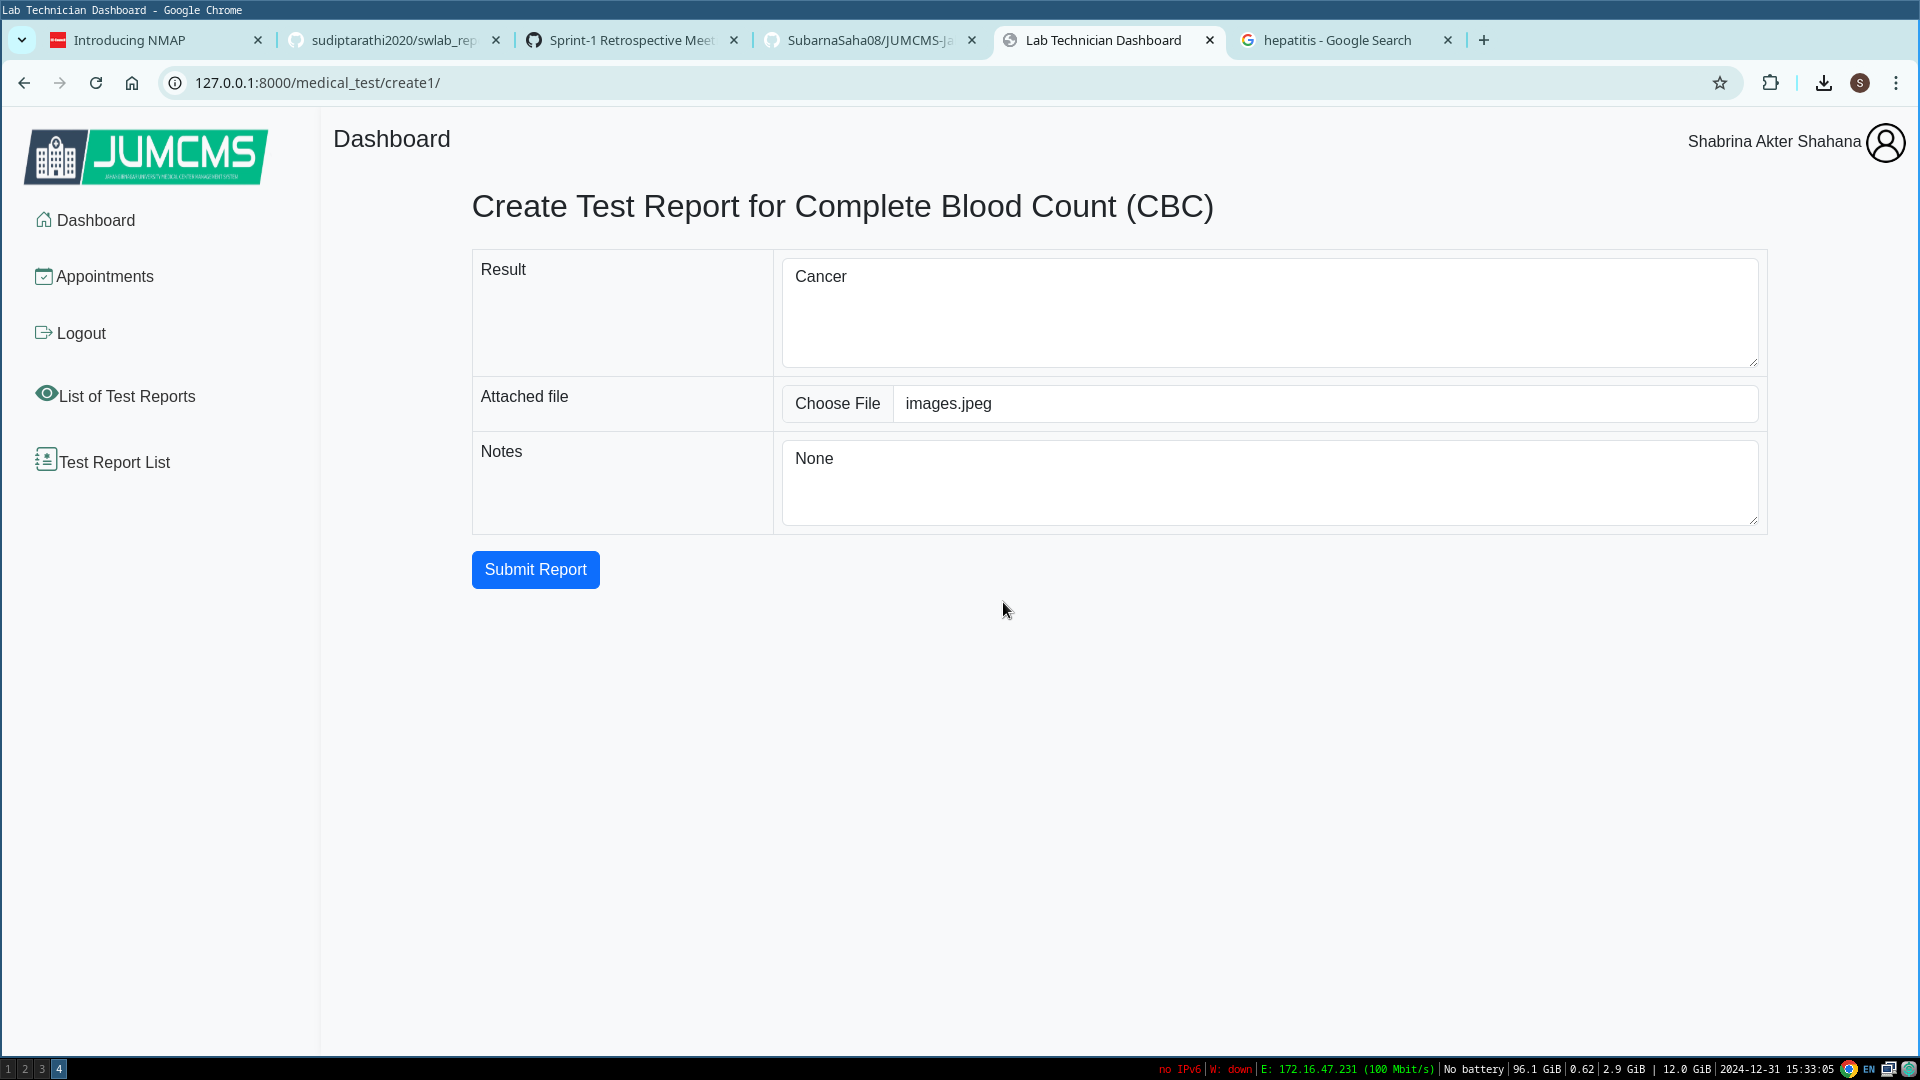
\includegraphics[width=1\textwidth]{images/sprintoutput07.png}
    \caption{Report Creation Form}
    \label{fig:reportform}
\end{figure}

\begin{figure}[H]
    \centering
    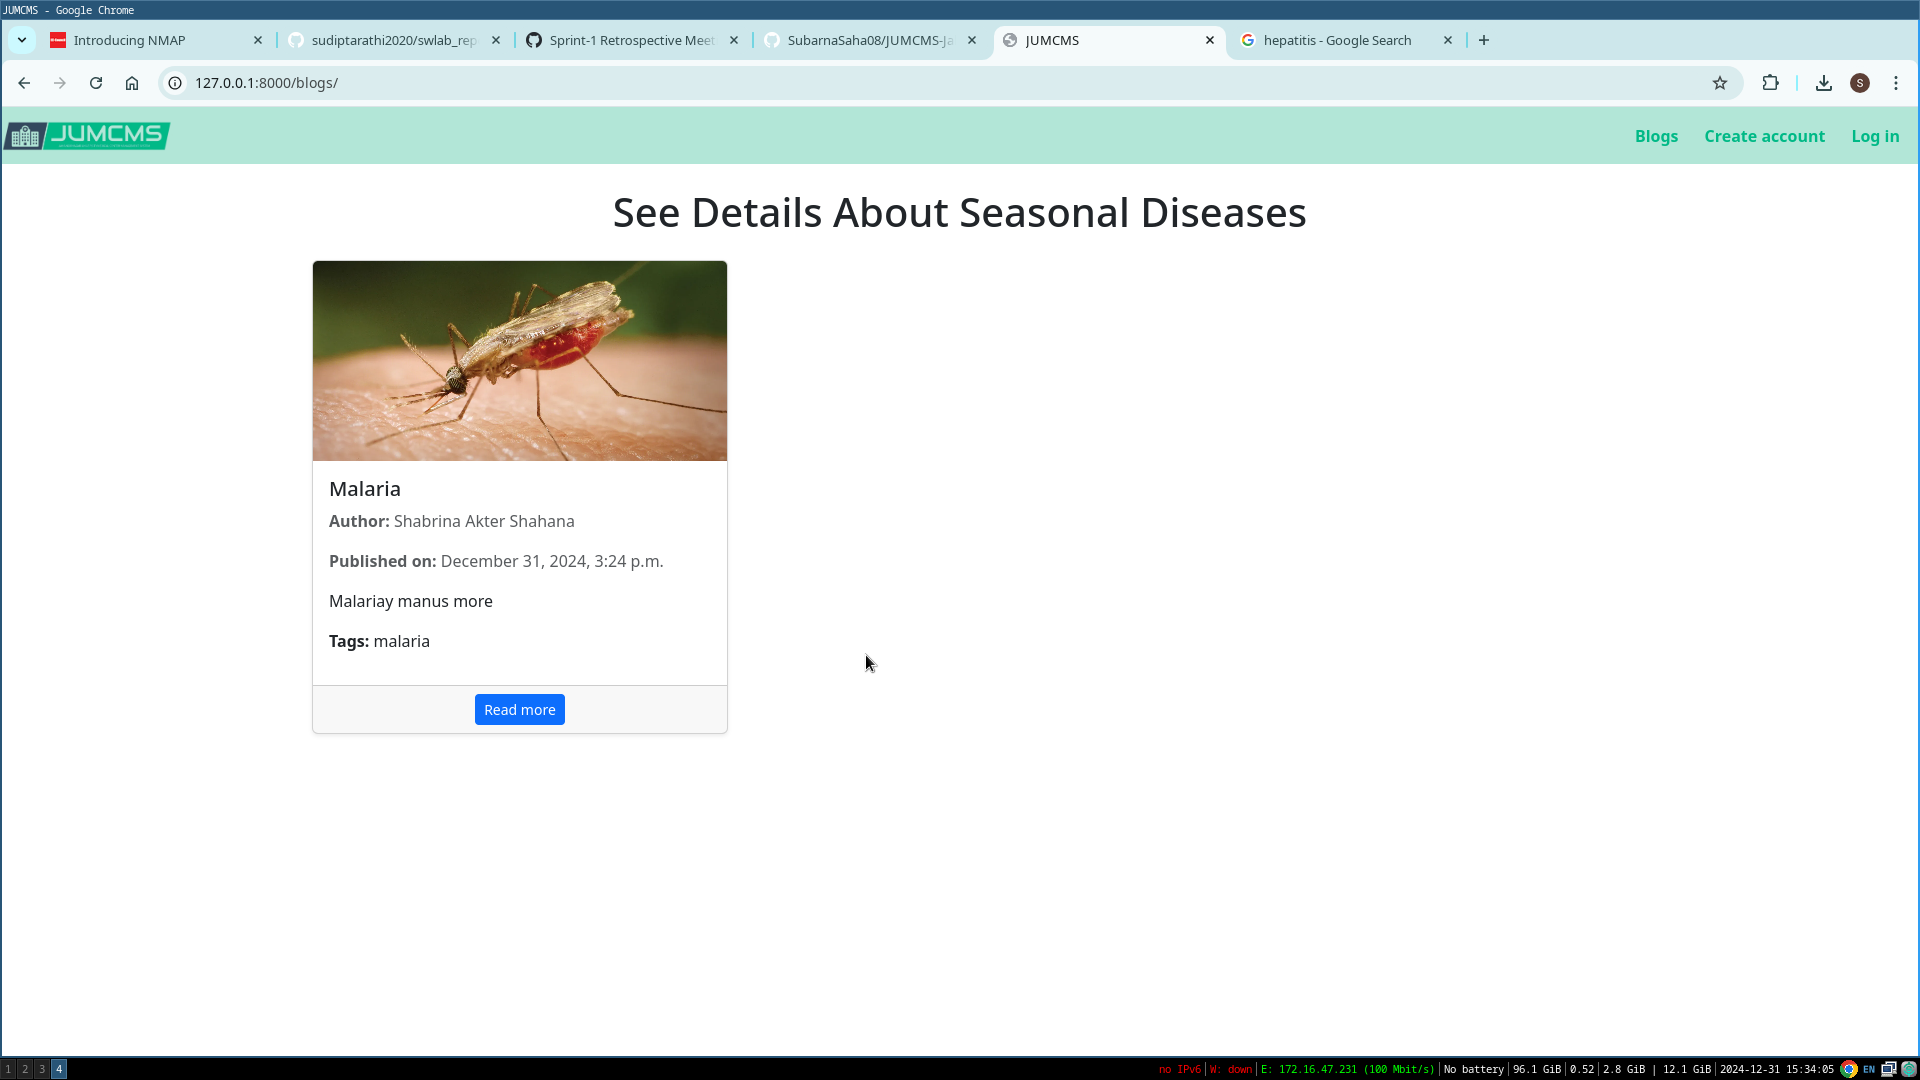
\includegraphics[width=1\textwidth]{images/sprintoutput08.png}
    \caption{Blogs}
    \label{fig:blogs}
\end{figure}

\begin{figure}[H]
    \centering
    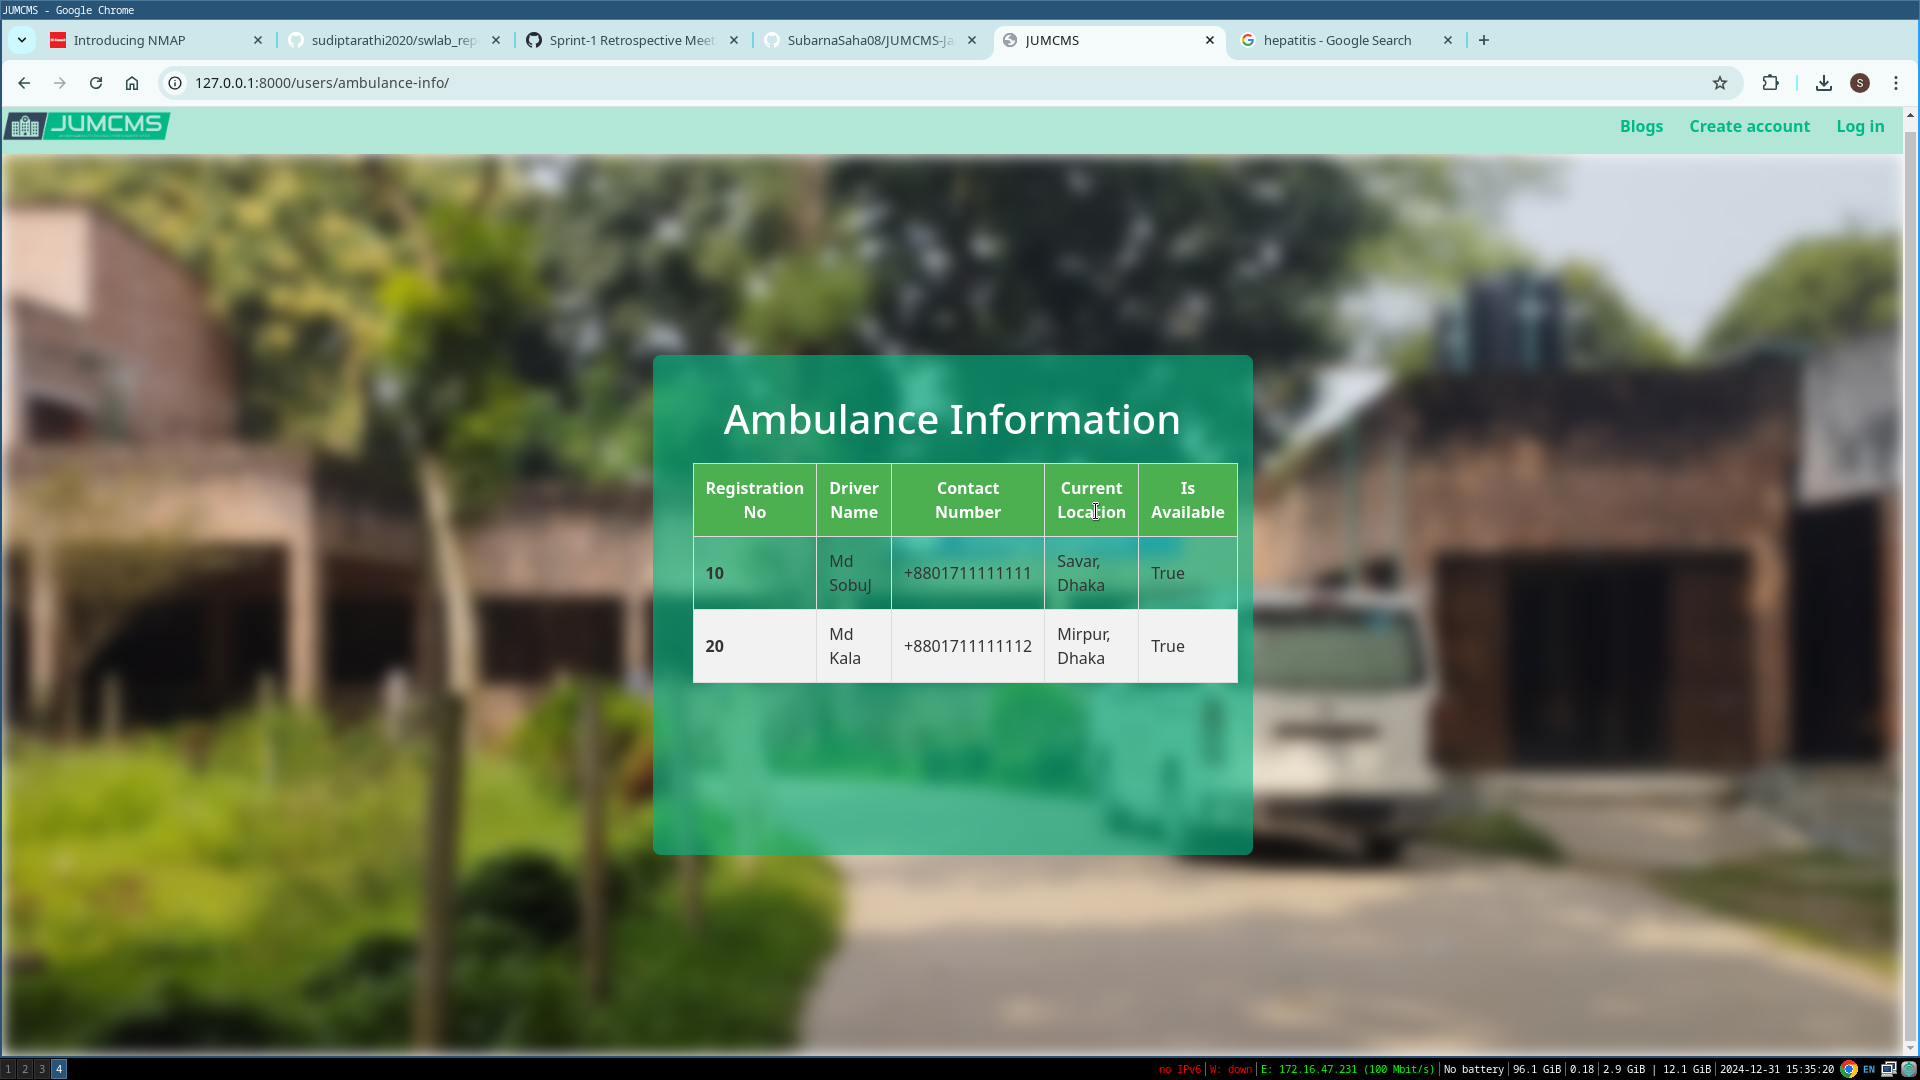
\includegraphics[width=1\textwidth]{images/sprintoutput09.png}
    \caption{Drivers information}
    \label{fig:driverinformation}
\end{figure}

\newpage
\section{Sprint Retrospective}

\end{document}
